\documentclass[12pt,twoside]{article}
\newcommand\independent{\protect\mathpalette{\protect\independenT}{\perp}}
\def\independenT#1#2{\mathrel{\rlap{$#1#2$}\mkern2mu{#1#2}}}


\usepackage{amsthm}
\usepackage{amsmath}
\usepackage{amssymb}
\usepackage{amsfonts}
\usepackage[margin=0.6in]{geometry}
\usepackage{enumerate}
\usepackage{relsize}
\usepackage{graphicx}
\usepackage{hyperref}
\usepackage{afterpage}
\usepackage{verbatim}
\usepackage{float}
\usepackage{amsthm}
\newtheorem{Theorem}{Theorem}
\newtheorem{Lemma}[Theorem]{Lemma}
\newtheorem{Definition}{Definition}
\newcommand{\mbf}{\mathbf}
\newcommand{\mrm}{\mathrm}
\usepackage{algorithm}
\usepackage[noend]{algpseudocode}
\newenvironment{centered}[0]{%

  \item[]}{\end{list}}

\setcounter{tocdepth}{1}
\newtheorem{theorem}{Theorem}

\title{Citadel Datathon at Berkeley}
\date{2/10/2017}
\author{Ming Jiao, Chuangwei Ruan, Xingyou Song, Yuzhou Zhao} 

\begin{document}
\nocite{*}

\maketitle
\abstract{The goal of this report is to predict the ridership for all locations for the new years 2016-2020.}

\tableofcontents
\section{Introduction (Non Technical)}
In our datathon challenge, we made initial investigations on the given data. We wanted to understand different relationships first, before making our question and analysis of the data. 
\subsection{Trips based on time} One initial observation was that intuitively, the uses of the train were based on the weekday and time, and that this followed a consistent trend throughout the years. For example, people generally used the train more during the hours for which people went and came back from work. Furthermore, the number of trains used were much higher during the weekdays than in the weekends. This generally supports the fact that people generally take the train for work mostly. We defined morning as 6-9 AM, evening as 6-8 PM, and every other time at other.
 
The following figure in figure 1 \ref{figure1} shows for example, that in those $2$ hours during, more than half of the trips taken compared to the other, were in the evening. Furthermore, the sum of the trips taken in the morning and evening are equal to the trips taken over all other times, even though the total time used for both is only 5 hours. 

Another observation is that people took the train far less during the weekends; the total trips used was less than half of the total trips used during a weekday. 


Another way of seeing this is in figure 2 \ref{figure2}, where the deviations in weekday/weekend trips follow a time-series.  

\subsection{Trips based on Location}
We also wanted to see which places most people used the train to travel to. Intuitively, we thought that perhaps most of the uses of the train are towards San Francisco, because there are more jobs and generally more population. The following figure 3 \ref{figure3} also supports this. \footnote{The SF stations were defined as the ones which cross the water towards the left isle, near the Civic Center}. We took each trip, and separated its ending destination and classified it as either in SF or not. As seen, there was a significant difference between the trips used; on average, there were around $40000$ more trips taken to SF than not. 



Another visualization we saw were the trips from each zip code to San Francisco, in figure 4 \ref{figure4}. We thought that perhaps there were more trips taken from different locations, and we wanted to see how distributed the trips made were. 
\subsection{Demographics} 
We wanted to see a time-trend for each location, and thus analyzed the total population, over many years, in figure 5 \ref{figure5}. Due to complexity and time constraints, we did not fine grain for more points for each zip code. However, as we can see, many of these zip codes show a consistent decrease or increase. However, some did not, and instead had periods of peaks and decreases. 

Other interesting facts about this analysis is that many of the zip codes that correspond to Silcon Valley have been steadily increasing. For example, zip codes 94030 and 94086 correspond to Silicon Valley, while 94128 corresponds to San Francisco Int'l Airport. Other places such as 94587 (Union City) corresponded to increasing population booms due to real estate.  


\section{Question} 
From the initial considerations, we saw that trips taken generally followed a very constant time series, and thus this was not interesting enough to investigate. However, what was more interesting was the trip amount distributions of the zip codes. We decided to investigate into this further, wanting to predict the trip amount for the future. This may be helpful for the industry to predict sales later on for business, as well as for resource allocation, such as producing more trains, or controlling the prices for maximal profit. 

In this section, we propose our question. Our question is: \textit{Given a zip code $z$, can we predict the number of trips used within that zip code in the future years 2017-2020? } \footnote{Note that if two stations are in the same zip code, we essentially will inherently sum them.}  Intuitively, a year's number of trips is based on the related parameters at the same time. Denote $Y_{t,z}$ to be the predicted value for the number of trips used at zip code $z$, at future year $t$. We only considered the zip codes $z$ for $Y_{t,z}$ that do contain a station. 

\subsection{General Considerations(Technical)} 

We considered many parameters, but the most significant associated examples to \textit{any} $z$ were: 
\begin{itemize}
\item Population $P_{t,z}$ 
\item Education level $E_{t,z}$ 
\item Average Income $I_{t,z}$
\item Previous year's trips, $Y_{t-1,z}, Y_{t-2,z}$ 
\end{itemize}   


Note that we appended the subscript $t$ to all of these parameters, because we saw that there was an increasing trend as a function of time. Understandably, for each of the parameters, we mainly only considered the data points of the past (2011- 2015). 

While we understood this may statistically speaking, generate a large risk due to small data points to train from, in real life, the trends of each of the parameters generally cannot change very much. Thus, we were more confident that we could predict those parameters with some guarentee of accuracy. 

However, we used 18 parameters in total for the prediction problem, 16 of which from demographic data, the zip code radius, and previous years.

Our classifer goes as follows: We first predict the time-dependent parameters from demographic data, and then take all of the population the set of zip codes within a radius of the specified zip code. We also used the previous year's data in our considerations.

\subsection{Technical Details }

\subsubsection{Time-Dependent Parameters}
For time-prediction, we could only use the demographics from 2011-2014. The only data we received were the demographic data per year, and thus we could only rely on 4 data points per zip code. We used a recency bias technique, in which if we had points $P_{2011,z},..., P_{2014,z}$, then we considered the differences $d_{i,z} = P_{2011+i, z} - P_{2010+i,z}$ and then took a weighted sum to predict the next difference between $P_{2015,z}$ and $P_{2016,z}$. For instance, we let $d_{4,z} = \frac{1}{6}d_{1,z} + \frac{1}{3} d_{2,z} + \frac{1}{2} d_{3,z}$ and predicted the next population as $d_{4,z}+ P_{2014,z}$. We could use a more sophisticated method from time-series analysis if we were given more data. 

\subsubsection{Classifer}
The predictors are the 16 parameters in demographics.csv, and the previous year's trip counts. We used an SVM-regression method, using the Gaussian basis kernel. 
We also used a Lasso method for linear classification as well. 
A brief introduction to these methods are found online, e.g. \url{https://www.mathworks.com/help/stats/understanding-support-vector-machine-regression.html?requestedDomain=www.mathworks.com}



Our code is inside the file we have sent. 
\subsubsection{Results}
Even though our time-varying data was not so refined, our predictor still achieved good results. In figure 6 \ref{figure6}, we compared our classifer's prediction to the actual trip counts for the 2015 year, and see very close predictions for each zip code. We normalized by taking the predicted/actual values and divided them by the standard deviation of the given data. 
For our algorithm in particular and its performance, our information selection criterion is shown in figure 7  \ref{figure7} and its Lasso path for coefficients are in figure 8 \ref{figure8}


Our data for estimation is included as well as a csv file, named "estimated demo"
\section{Appendix} 
The next pages include our figures that we referenced from earlier. The files:
"estimated demo" predicts the demographic for 2015-2020. The "exploratory data analysis" outputted the figures. The "prediction" file is the code for the model. The "results" is the final result for the ridership prediction.




\begin{figure}[p] \label{figure1} 
\centerline{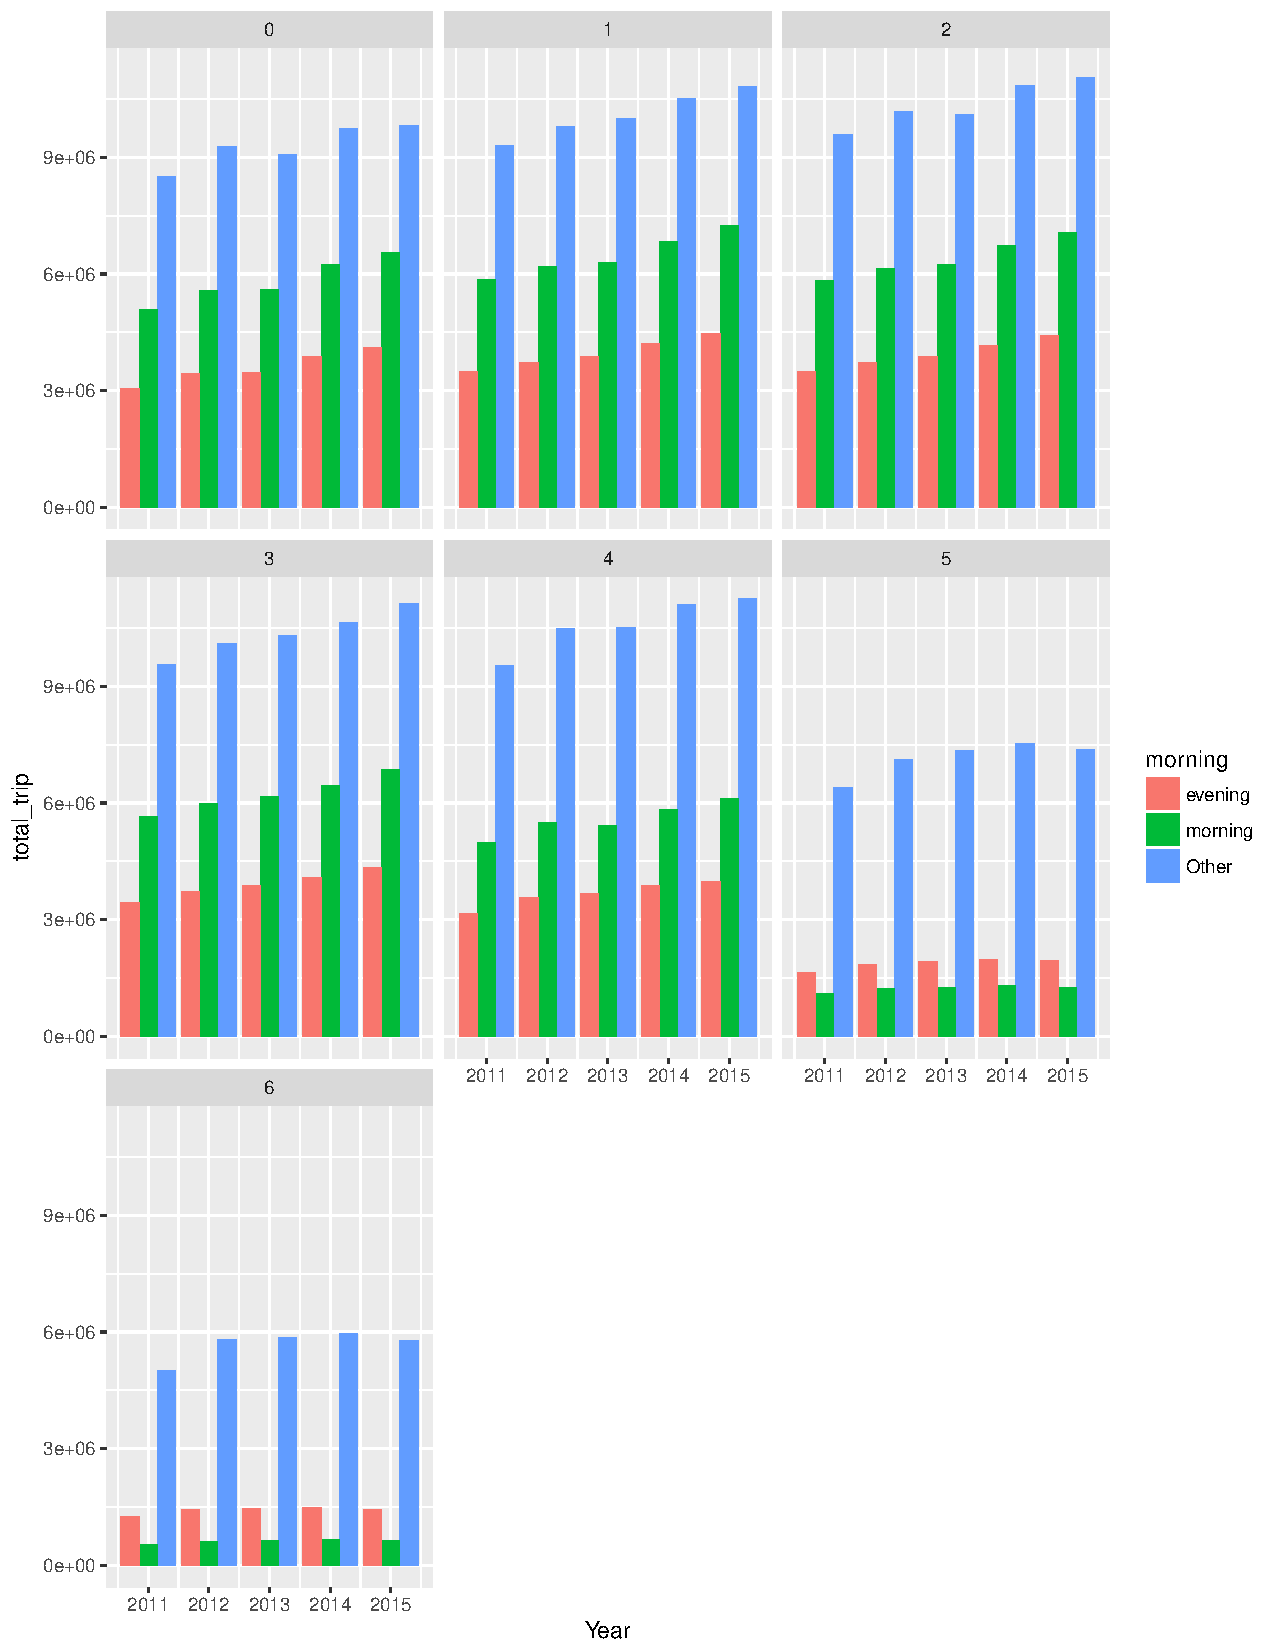
\includegraphics[scale=0.6]{Rplot01.pdf}}
\caption{A histogram of the total trips taken per year, based on evening and morning, separated by weekdays. (5 is Saturday, 6 is Sunday)  }
\end{figure}

\newpage
\begin{figure} \label{figure2} 
\centerline{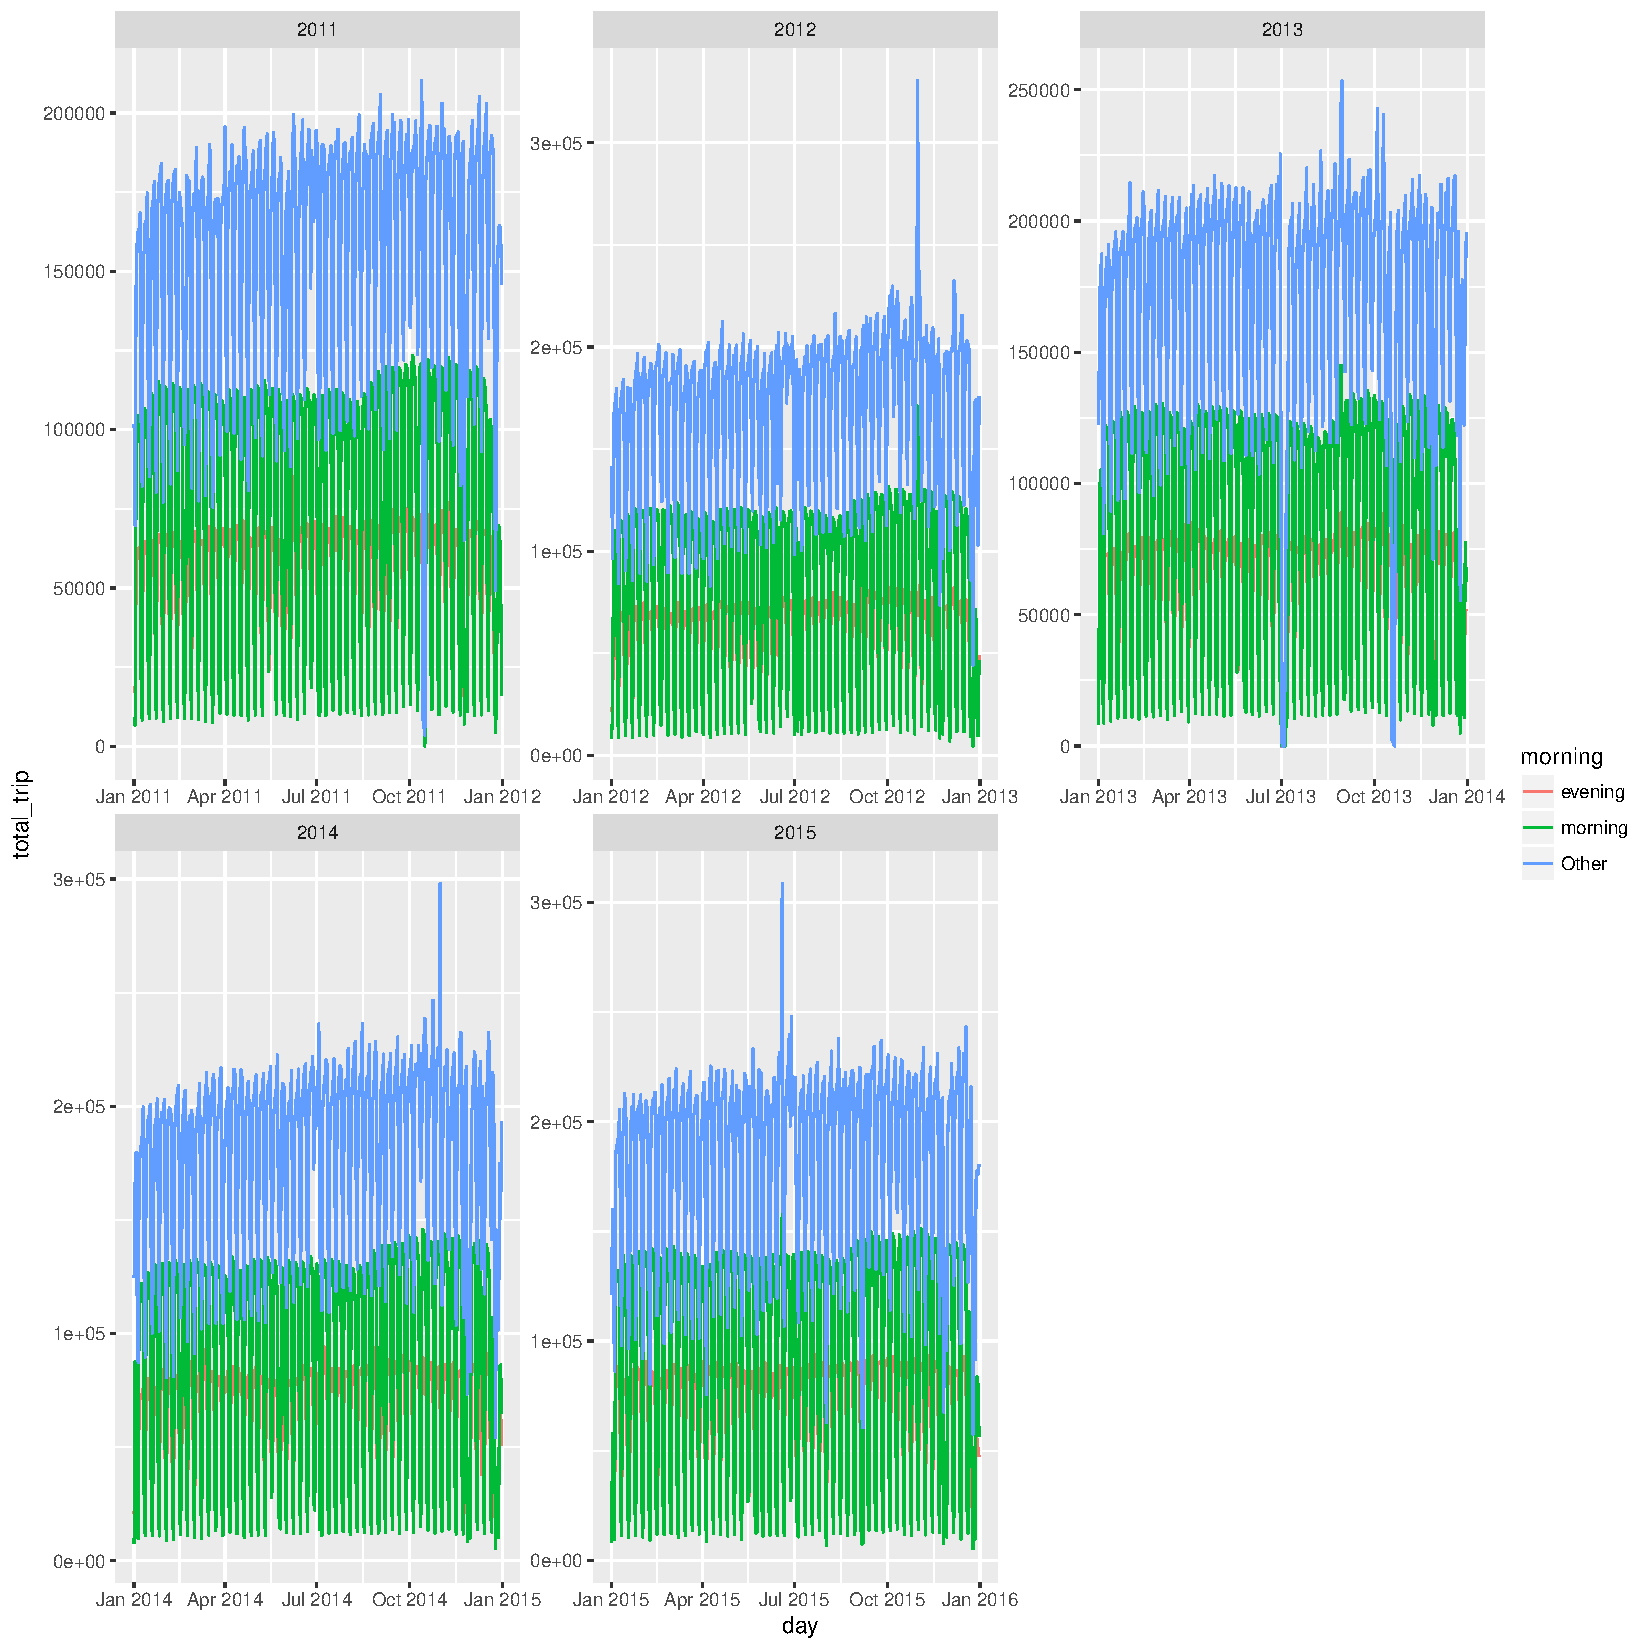
\includegraphics[scale=0.6]{Rplot02.pdf}}
\caption{A graph plot of the varying trips taken over many years.  }
\end{figure}
\newpage
\begin{figure} \label{figure3} 
\centerline{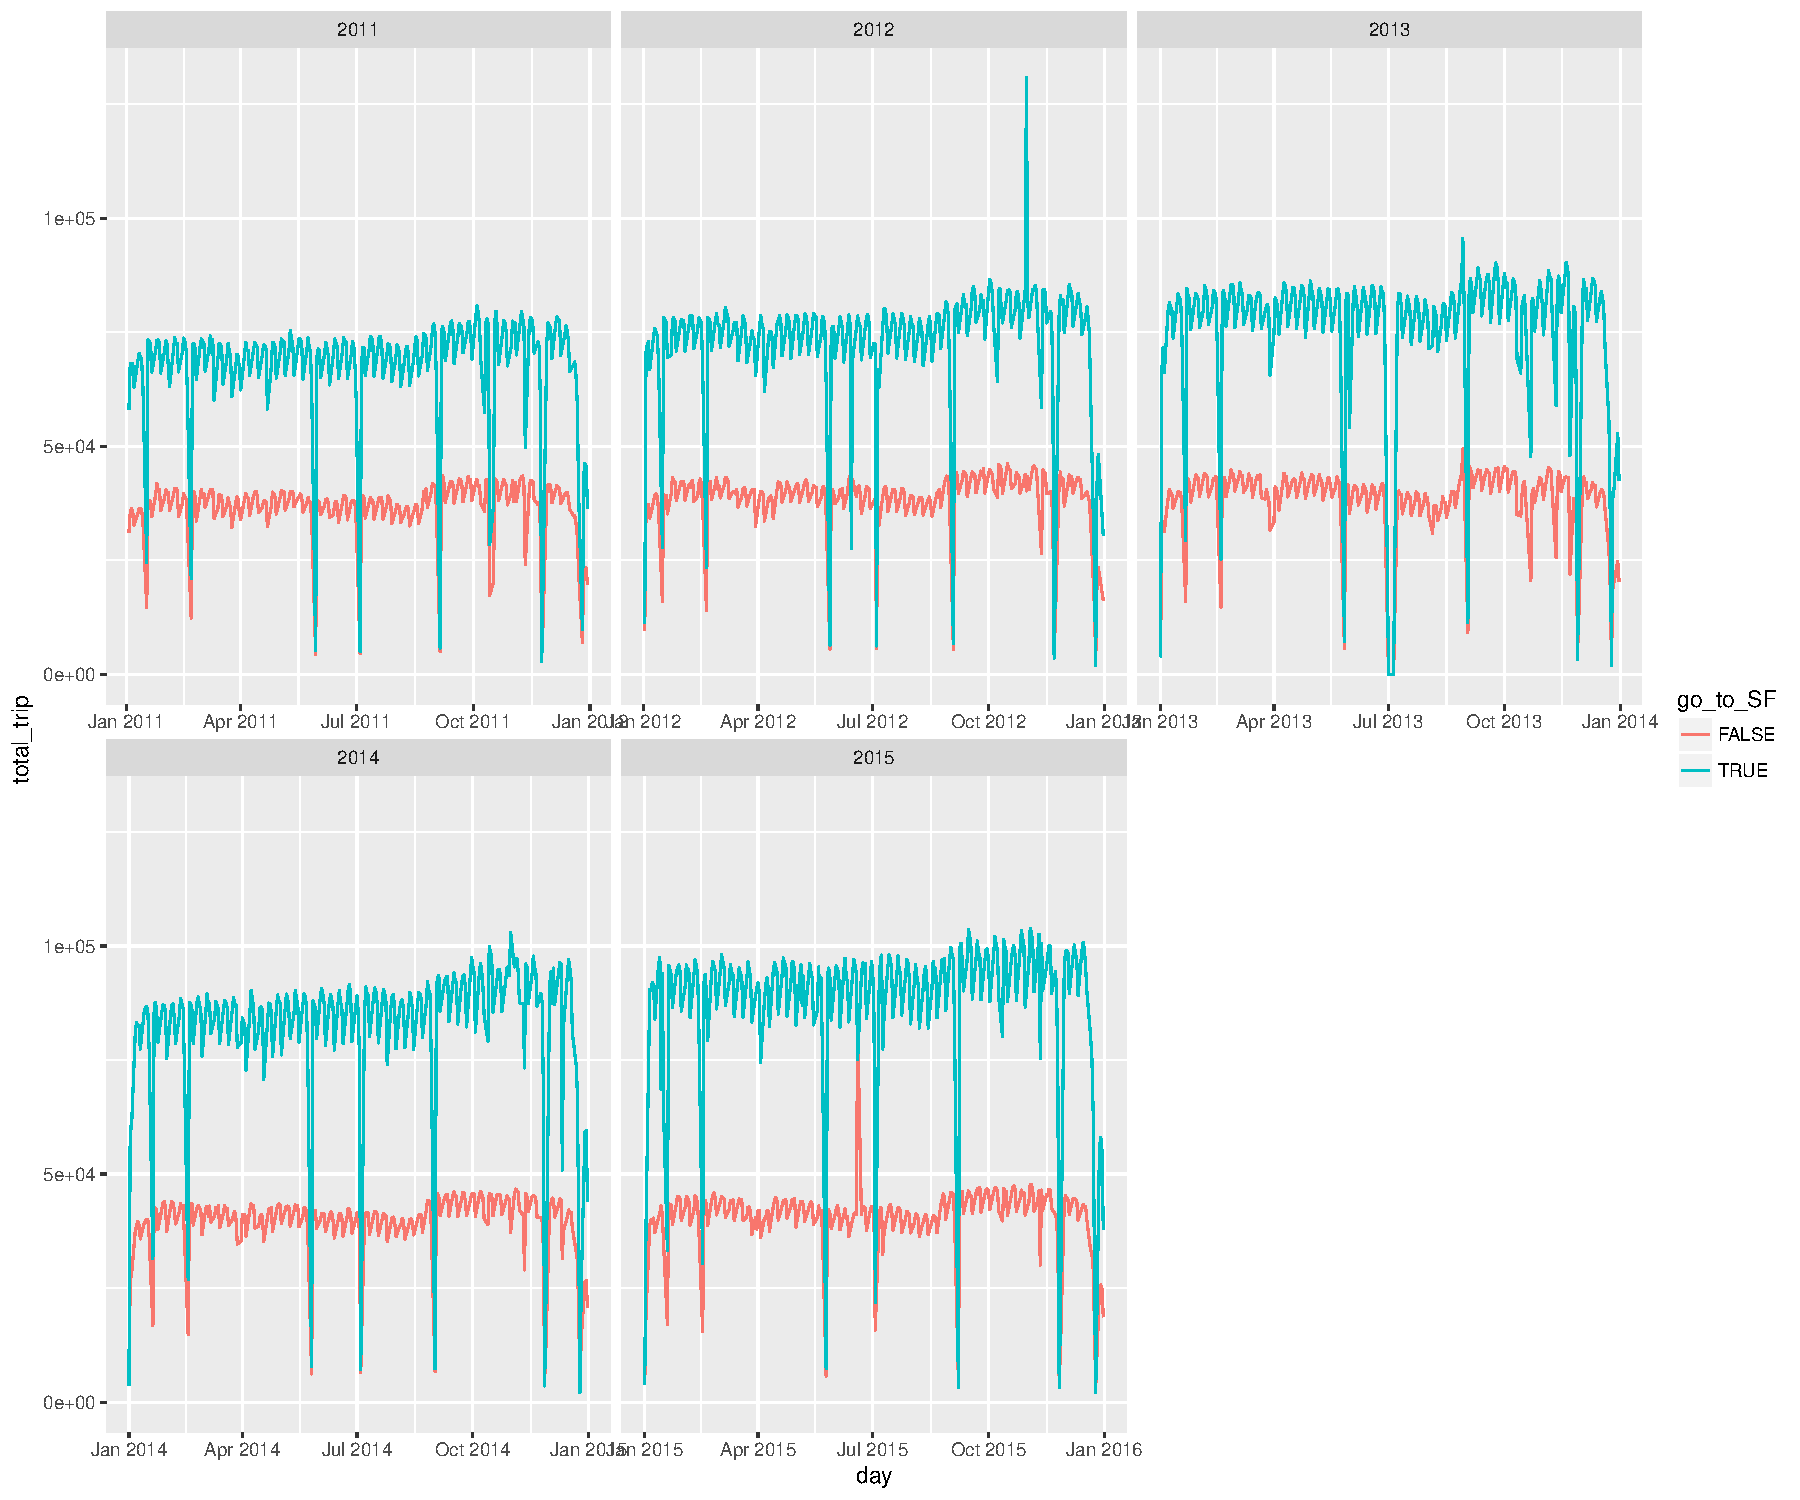
\includegraphics[scale=0.6]{Rplot03.pdf}}
\caption{A graph of which trips went to SF, and which did not. }
\end{figure} 
\newpage
\begin{figure} \label{figure4} 
\centerline{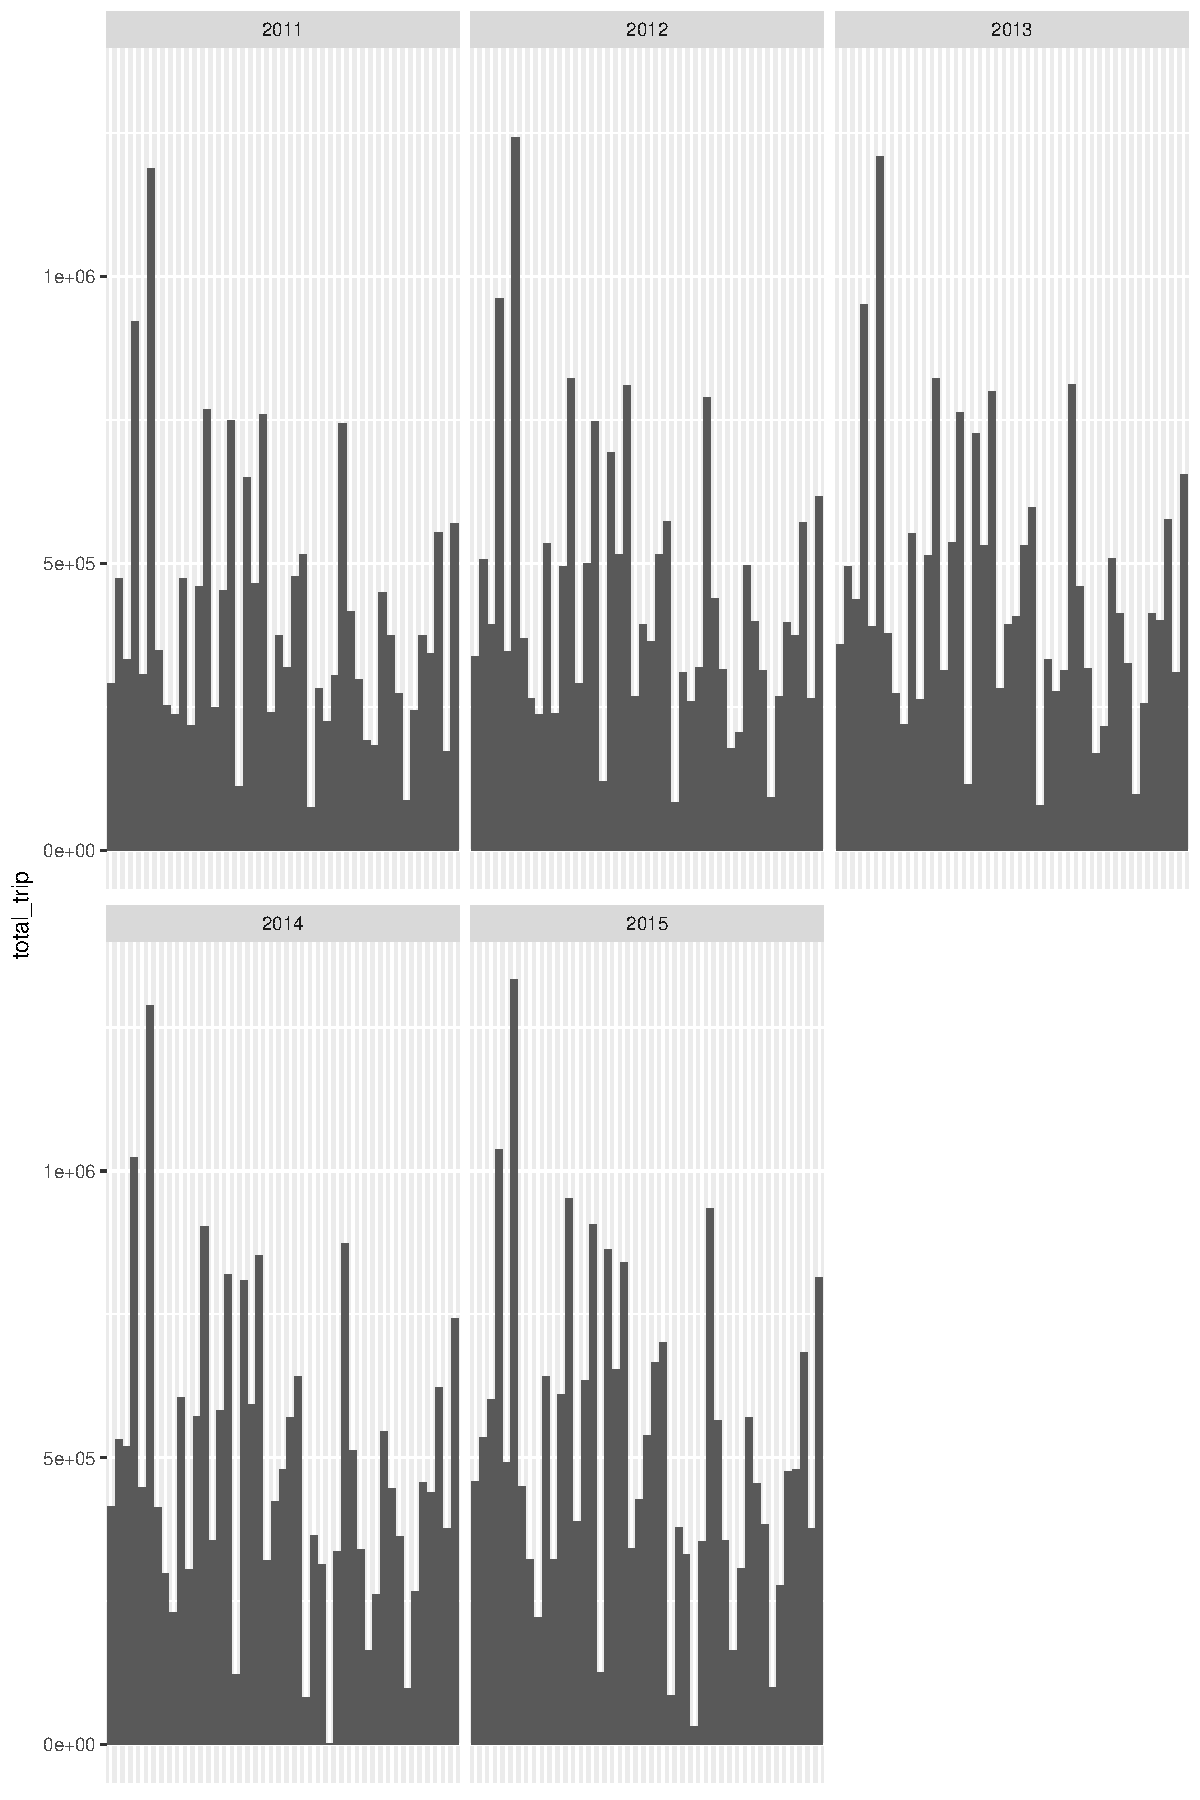
\includegraphics[scale=0.6]{Rplot04.pdf}}
\caption{A graph of all the possible zip codes. The x-axis does NOT represent each zip code within some range, but rather it is a random permutation over all zip codes.  }
\end{figure} 
\begin{figure} \label{figure5} 
\centerline{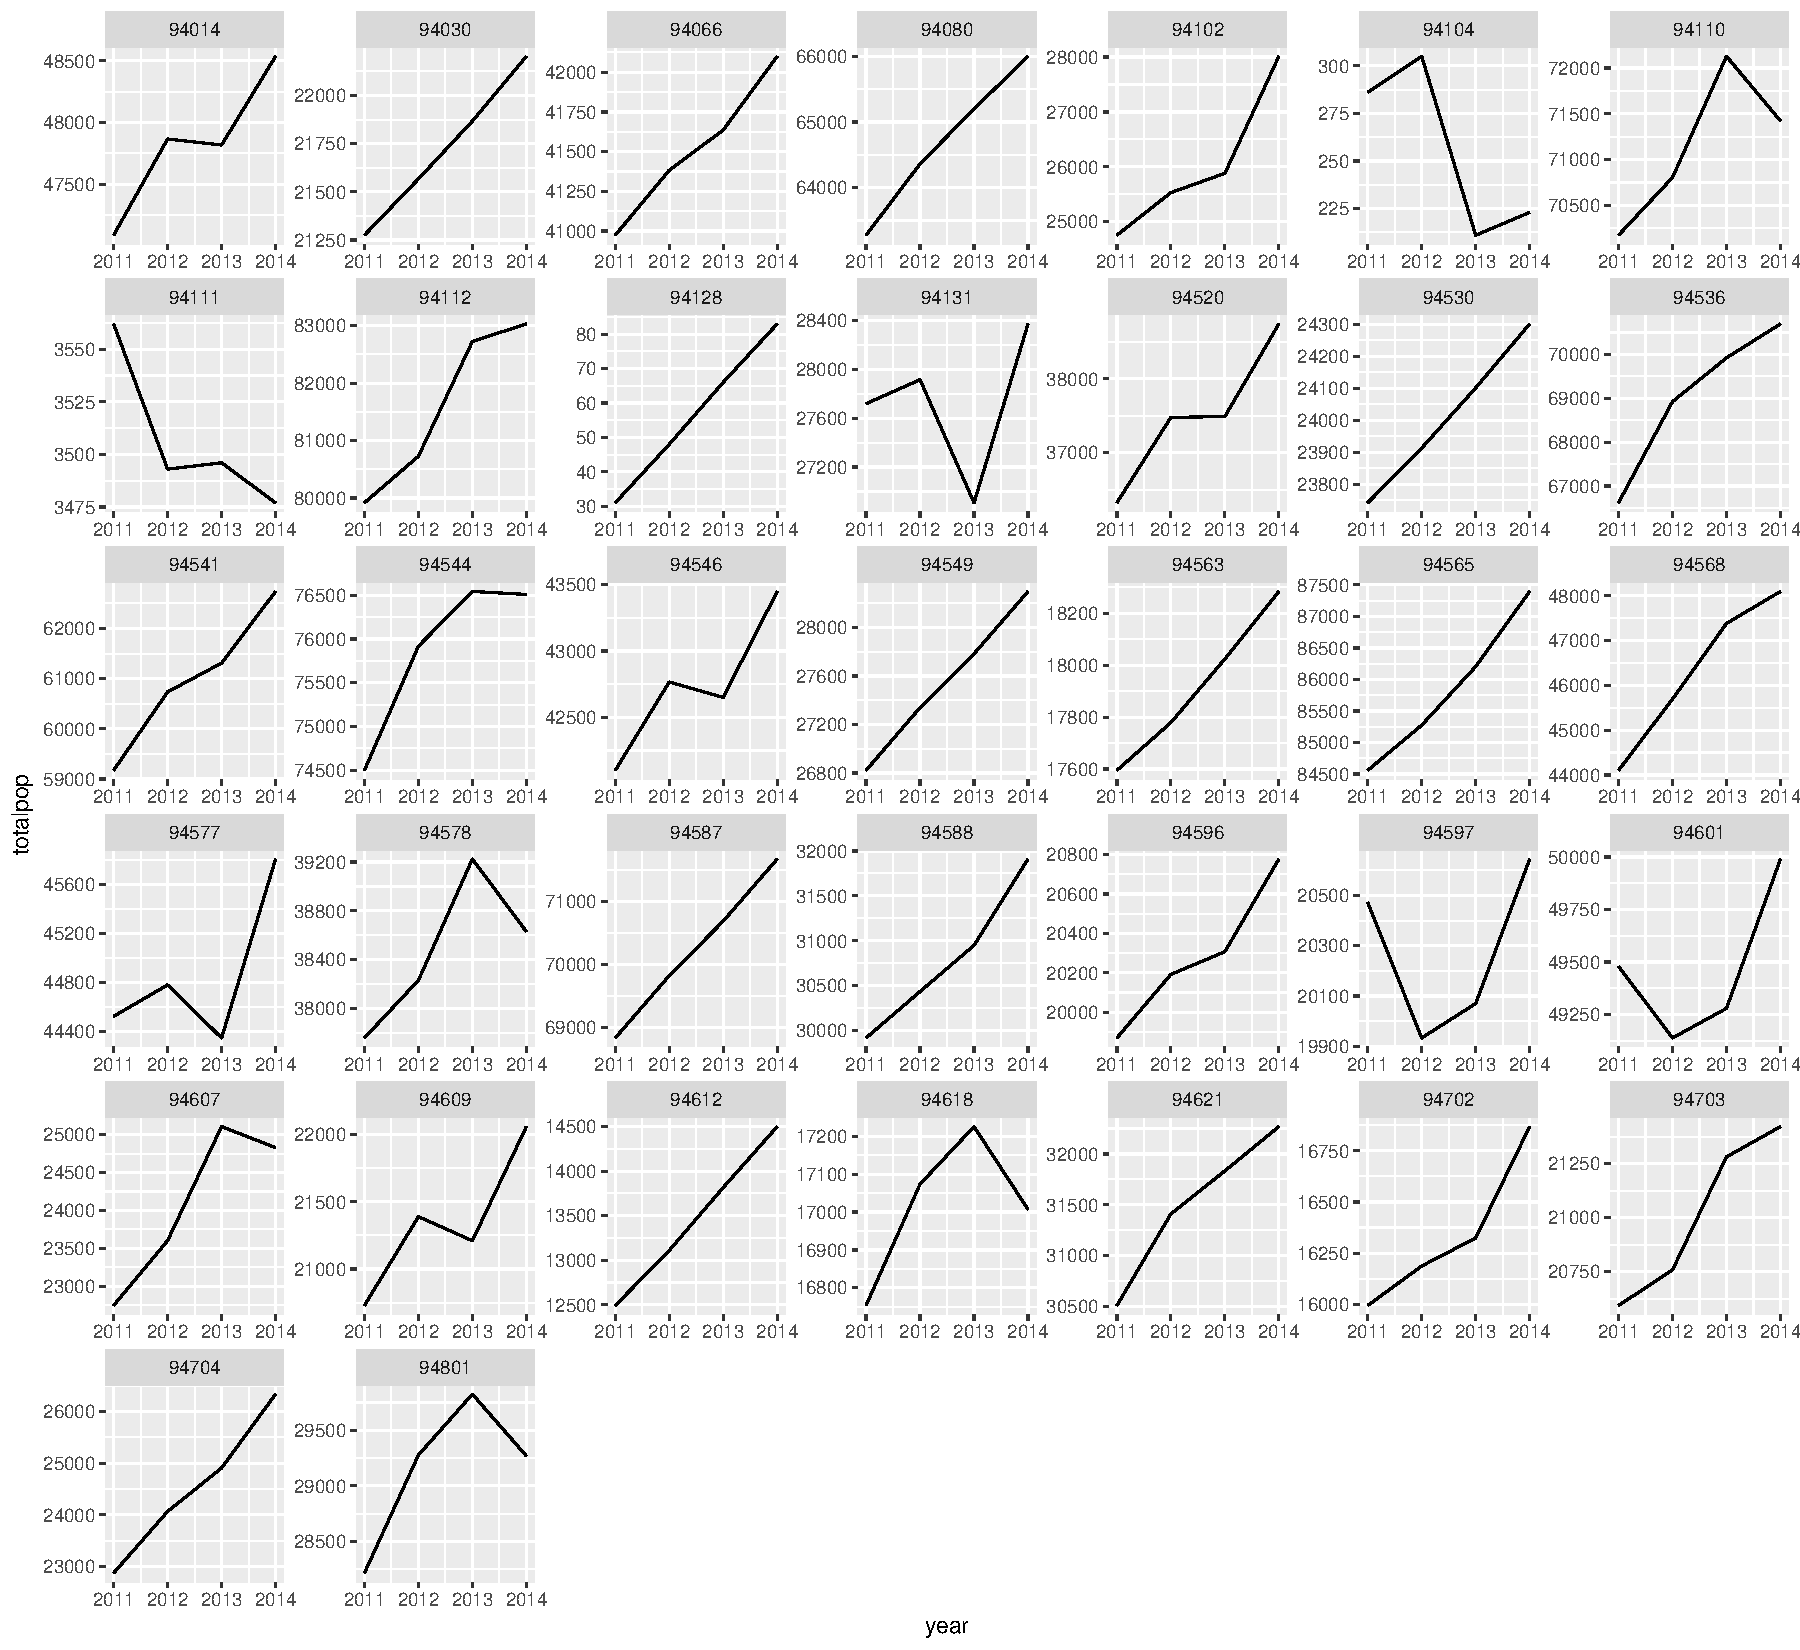
\includegraphics[scale=0.6]{Rplot05.pdf}}
\caption{A graph of all the possible zip codes, and a plot over time of trips taken out of these zip codes.  }
\end{figure} 
\begin{figure} \label{figure6} 
\centerline{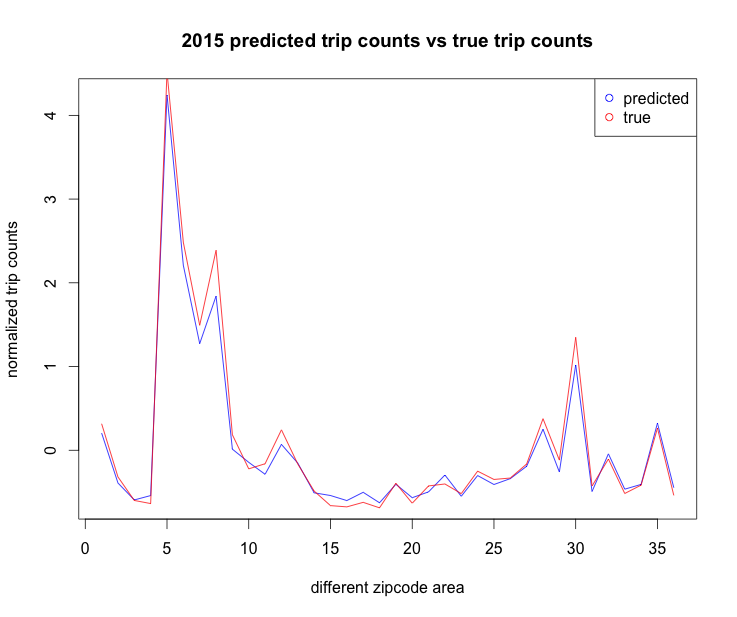
\includegraphics[scale=0.6]{predicted2015.png}}
\caption{A graph of the predicted and actual normalized trip counts for each zip code }
\end{figure} 

\begin{figure} \label{figure7} 
\centerline{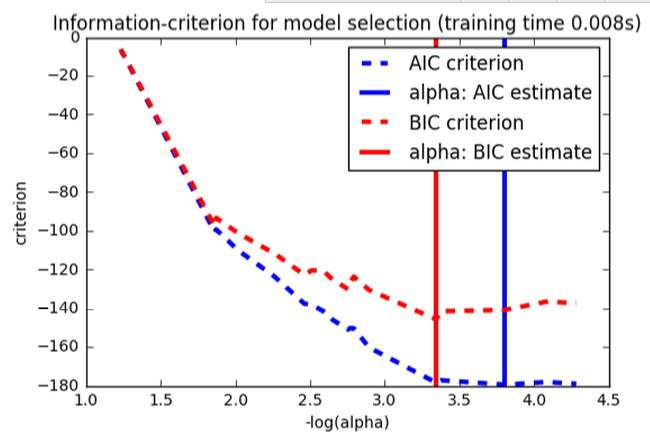
\includegraphics[scale=0.8]{alpha.jpg}}
\caption{Graph of the Akaike information criterion for our model. }
\end{figure}

\begin{figure} \label{figure8} 
\centerline{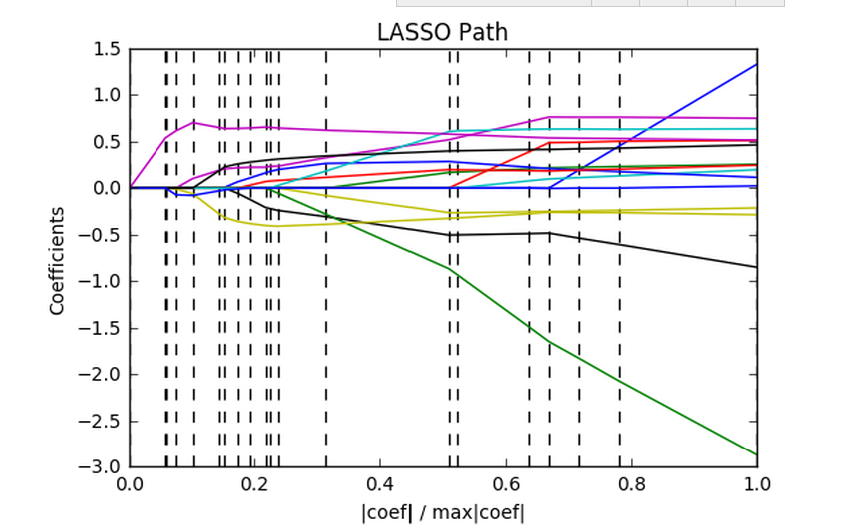
\includegraphics[scale=0.8]{coefficients.jpg}}
\caption{Lasso path for coefficients in our classifier. }
\end{figure}
\newpage 

\end{document}